\documentclass[11pt]{article}
\usepackage{amsmath}
\usepackage{amssymb}
\usepackage{graphicx}
\usepackage{tabularx}
\usepackage{fancyhdr}
\usepackage{lastpage}

% Page layout
\usepackage[top=1in, bottom=1in, left=1in, right=1in]{geometry}

% Header and footer
\pagestyle{fancy}
\fancyhf{}
\rfoot{Page \thepage}
\renewcommand{\headrulewidth}{0pt}

% Modified Question command with left-aligned number
\newcommand{\questiona}[2]{
    \noindent\textbf{Q#2.} #1 \hfill \textbf{[1 Mark]}
}

\newcommand{\questionb}[2]{
    \noindent\textbf{Q#2.} #1 \hfill \textbf{[2 Marks]}
}

\begin{document}

% Title section with horizontal line
\begin{center}
    \Large\textbf{GATE 2018 - Geology and Geophysics (GG)} \\
    \large\textbf{General Aptitude and Technical Questions} \\
    \rule{\textwidth}{0.5pt} % Horizontal line below heading
\end{center}

\vspace{0.5cm}

% General Aptitude Section
\section*{General Aptitude}

\questiona{“When she fell down the \_\_\_\_\_, she received many \_\_\_\_\_ but little help.”}{1}
\begin{enumerate}
    \item[(A)] stairs, stares
    \item[(B)] stairs, stairs
    \item[(C)] stares, stairs
    \item[(D)] stares, stares
\end{enumerate}
\vspace{0.5cm}

\questiona{In spite of being warned repeatedly, he failed to correct his \_\_\_\_\_ behaviour.}{2}
\begin{enumerate}
    \item[(A)] rational
    \item[(B)] reasonable
    \item[(C)] errant
    \item[(D)] good
\end{enumerate}
\vspace{0.5cm}

\questiona{For \( 0 \leq x \leq 2\pi \), \(\sin x\) and \(\cos x\) are both decreasing functions in the interval \_\_\_\_\_.}{3}
\begin{enumerate}
    \item[(A)] \( \left(0, \frac{\pi}{2} \right) \)
    \item[(B)] \( \left( \frac{\pi}{2}, \pi \right) \)
    \item[(C)] \( \left( \pi, \frac{3\pi}{2} \right) \)
    \item[(D)] \( \left( \frac{3\pi}{2}, 2\pi \right) \)
\end{enumerate}
\vspace{0.5cm}

\questiona{The area of an equilateral triangle is \(\sqrt{3}\). What is the perimeter of the triangle?}{4}
\begin{enumerate}
    \item[(A)] 2
    \item[(B)] 4
    \item[(C)] 6
    \item[(D)] 8
\end{enumerate}
\vspace{0.5cm}

\questiona{Arrange the following three-dimensional objects in the descending order of their volumes: (i) A cuboid with dimensions 10 cm, 8 cm and 6 cm, (ii) A cube of side 8 cm, (iii) A cylinder with base radius 7 cm and height 7 cm, (iv) A sphere of radius 7 cm}{5}
\begin{enumerate}
    \item[(A)] (i), (ii), (iii), (iv)
    \item[(B)] (ii), (i), (iv), (iii)
    \item[(C)] (iii), (ii), (i), (iv)
    \item[(D)] (iv), (iii), (ii), (i)
\end{enumerate}
\vspace{0.5cm}

\questionb{An automobile travels from city A to city B and returns to city A by the same route. The speed of the vehicle during the onward and return journeys were constant at 60 km/h and 90 km/h, respectively. What is the average speed in km/h for the entire journey?}{6}
\begin{enumerate}
    \item[(A)] 72
    \item[(B)] 73
    \item[(C)] 74
    \item[(D)] 75
\end{enumerate}
\vspace{0.5cm}

\questionb{A set of 4 parallel lines intersect with another set of 5 parallel lines. How many parallelograms are formed?}{7}
\begin{enumerate}
    \item[(A)] 20
    \item[(B)] 48
    \item[(C)] 60
    \item[(D)] 72
\end{enumerate}
\vspace{0.5cm}

\questionb{To pass a test, a candidate needs to answer at least 2 out of 3 questions correctly. A total of 6,30,000 candidates appeared for the test. Question A was correctly answered by 3,30,000 candidates. Question B was answered correctly by 2,50,000 candidates. Question C was answered correctly by 2,60,000 candidates. Both questions A and B were answered correctly by 1,00,000 candidates. Both questions B and C were answered correctly by 90,000 candidates. Both questions A and C were answered correctly by 80,000 candidates. If the number of students answering all questions correctly is the same as the number answering none, how many candidates failed to clear the test?}{8}
\begin{enumerate}
    \item[(A)] 30,000
    \item[(B)] 2,70,000
    \item[(C)] 3,90,000
    \item[(D)] 4,20,000
\end{enumerate}
\vspace{0.5cm}

\questionb{If \( x^2 + x - 1 = 0 \), what is the value of \( x^4 + \frac{1}{x^4} \)?}{9}
\begin{enumerate}
    \item[(A)] 1
    \item[(B)] 5
    \item[(C)] 7
    \item[(D)] 9
\end{enumerate}
\vspace{0.5cm}

\questionb{In a detailed study of annual crow births in India, it was found that there was relatively no growth during the period 2002 to 2004 and a sudden spike from 2004 to 2005. In another unrelated study, it was found that the revenue from cracker sales in India which remained fairly flat from 2002 to 2004, saw a sudden spike in 2005 before declining again in 2006. The solid line in the graph below refers to annual sale of crackers and the dashed line refers to the annual crow births in India. Choose the most appropriate inference from the above data. \\ \\ 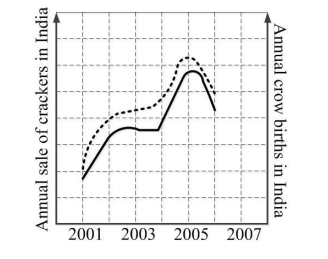
\includegraphics[width=0.5\textwidth]{figures/10}}{10}
\begin{enumerate}
    \item[(A)] There is a strong correlation between crow birth and cracker sales.
    \item[(B)] Cracker usage increases crow birth rate.
    \item[(C)] If cracker sale declines, crow birth will decline.
    \item[(D)] Increased birth rate of crows will cause an increase in the sale of crackers.
\end{enumerate}
\vspace{0.5cm}

\section*{Technical Section}

\questiona{Which one of the following periods has the longest time duration?}{1}
\begin{enumerate}
    \item[(A)] Ordovician
    \item[(B)] Cretaceous
    \item[(C)] Jurassic
    \item[(D)] Silurian
\end{enumerate}
\vspace{0.5cm}

\questiona{A siliciclastic sedimentary rock consisting predominantly of the same type of gravel-sized clasts is called}{2}
\begin{enumerate}
    \item[(A)] Polymict conglomerate
    \item[(B)] Arkose
    \item[(C)] Oligomict conglomerate
    \item[(D)] Petromict conglomerate
\end{enumerate}
\vspace{0.5cm}

\questiona{Brown coal that has high moisture content and commonly retains many of the original wood fragments is called}{3}
\begin{enumerate}
    \item[(A)] Anthracite
    \item[(B)] Bituminous coal
    \item[(C)] Lignite
    \item[(D)] Peat
\end{enumerate}
\vspace{0.5cm}

\questiona{The speed of revolution of the Earth around the Sun is}{4}
\begin{enumerate}
    \item[(A)] maximum at Perihelion
    \item[(B)] minimum at Perihelion
    \item[(C)] maximum at Aphelion
    \item[(D)] equal at Aphelion and Perihelion
\end{enumerate}
\vspace{0.5cm}

\questiona{The geometrical factor for the following electrode configuration is}{5}
\begin{center}
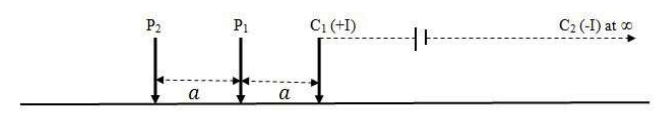
\includegraphics[width=0.8\textwidth]{figures/5.png}
\end{center}
\begin{enumerate}
    \item[(A)] \( \pi a \)
    \item[(B)] \( 2\pi a \)
    \item[(C)] \( 3\pi a \)
    \item[(D)] \( 4\pi a \)
\end{enumerate}
\vspace{0.5cm}

\questiona{Which one of the following geophysical methods uses the physical property ‘Dielectric Constant’?}{6}
\begin{enumerate}
    \item[(A)] Gravity
    \item[(B)] Ground Penetrating Radar
    \item[(C)] Seismic
    \item[(D)] Self-Potential
\end{enumerate}
\vspace{0.5cm}

\questiona{Pascal second is a unit of}{7}
\begin{enumerate}
    \item[(A)] seepage force
    \item[(B)] dynamic viscosity
    \item[(C)] kinematic viscosity
    \item[(D)] permeability
\end{enumerate}
\vspace{0.5cm}

\questiona{Which one of the following statements is CORRECT?}{8}
\begin{enumerate}
    \item[(A)] Strength of a rock decreases with increase in confining pressure.
    \item[(B)] Strength of a rock increases with increase in temperature.
    \item[(C)] Strength of a rock increases with increase in strain rate.
    \item[(D)] Strength of a rock increases with increase in pore water pressure.
\end{enumerate}
\vspace{0.5cm}

\questiona{The geomorphic feature ‘horns’ are formed by}{9}
\begin{enumerate}
    \item[(A)] wind erosion
    \item[(B)] river erosion
    \item[(C)] wind deposition
    \item[(D)] glacial erosion
\end{enumerate}
\vspace{0.5cm}

\questiona{A melanocratic porphyritic rock containing phenocrysts of biotite, with feldspar restricted to the groundmass, is called}{10}
\begin{enumerate}
    \item[(A)] trachyte
    \item[(B)] dacite
    \item[(C)] andesite
    \item[(D)] lamprophyre
\end{enumerate}
\vspace{0.5cm}

\questiona{The supercontinent that existed in the late Mesoproterozoic to early Neoproterozoic time was}{11}
\begin{enumerate}
    \item[(A)] Kenorland
    \item[(B)] Columbia
    \item[(C)] Rodinia
    \item[(D)] Pangaea
\end{enumerate}
\vspace{0.5cm}

\questiona{The figure below shows the triple junction between three plates A, B and C. The boundary between the plates A and B is a ridge with a half-spreading rate of 4 cm/year. The A-C and B-C boundaries are collinear and orthogonal to the A-B ridge. The A-C boundary is a dextral transform fault with a relative velocity of 6 cm/year. The boundary between plates B and C is a}{12}
\begin{center}
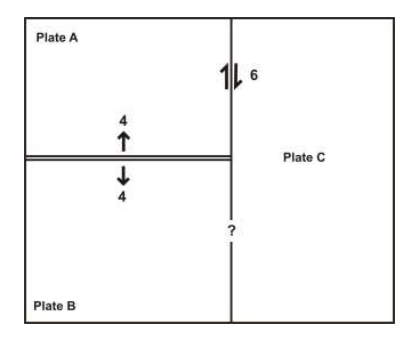
\includegraphics[width=0.5\textwidth]{figures/12}
\end{center}
\begin{enumerate}
    \item[(A)] dextral transform fault with a relative velocity of 10 cm/year
    \item[(B)] dextral transform fault with a relative velocity of 2 cm/year
    \item[(C)] sinistral transform fault with a relative velocity of 2 cm/year
    \item[(D)] sinistral transform fault with a relative velocity of 6 cm/year
\end{enumerate}
\vspace{0.5cm}

\questiona{A rock follows Mohr-Coulomb failure criterion. Which one of the Mohr-Coulomb failure envelopes shown below allows failure of the rock under stress state Y, but not under stress state X?}{13}
\begin{center}
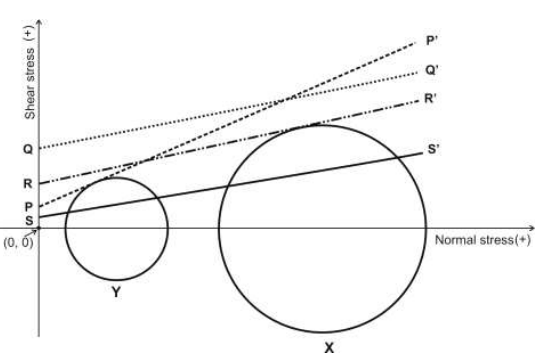
\includegraphics[width=0.5\textwidth]{figures/13}
\end{center}
\begin{enumerate}
    \item[(A)] PP’
    \item[(B)] QQ’
    \item[(C)] RR’
    \item[(D)] SS’
\end{enumerate}
\vspace{0.5cm}

\questiona{The maximum and the minimum principal stresses are denoted by \(\sigma_1\) and \(\sigma_3\), respectively. The differential stress can have an absolute value greater than \(\sigma_1\) when}{14}
\begin{enumerate}
    \item[(A)] \(\sigma_1\) and \(\sigma_3\) are both compressive
    \item[(B)] \(\sigma_1\) is compressive and \(\sigma_3\) is tensile
    \item[(C)] \(\sigma_1\) and \(\sigma_3\) are equal
    \item[(D)] \(\sigma_1\) and \(\sigma_3\) are both tensile
\end{enumerate}
\vspace{0.5cm}

\questiona{The geoid can be best defined as}{15}
\begin{enumerate}
    \item[(A)] an oblate spheroid that best approximates the shape of the earth
    \item[(B)] a surface over which the value of gravity is constant
    \item[(C)] the physical surface of the earth
    \item[(D)] an equipotential surface of gravity of the earth
\end{enumerate}
\vspace{0.5cm}

\questiona{For a layered isotropic medium with a flat horizontal free surface, match the wave types listed in Group-I with their corresponding polarizations listed in Group II.}{16}
\begin{center}
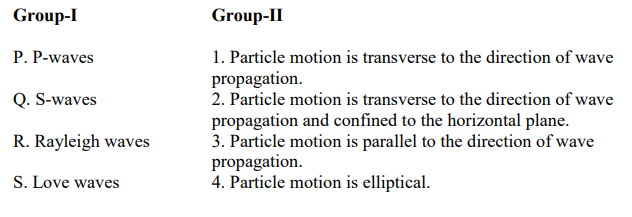
\includegraphics[width=0.8\textwidth]{figures/16.png}
\end{center}
\begin{enumerate}
    \item[(A)] P-1; Q-3; R-4; S-2
    \item[(B)] P-3; Q-1; R-4; S-2
    \item[(C)] P-3; Q-1; R-2; S-4
    \item[(D)] P-2; Q-3; R-1; S-4
\end{enumerate}
\vspace{0.5cm}

\questiona{A ‘gentle’ fold with an interlimb angle equal to \(160^\circ\) appears tight (apparent interlimb angle equal to \(20^\circ\)) in horizontal section. According to the plunge of the fold axis, it can also be classified as}{17}
\begin{enumerate}
    \item[(A)] horizontal fold
    \item[(B)] gently plunging fold
    \item[(C)] steeply plunging fold
    \item[(D)] vertical fold
\end{enumerate}
\vspace{0.5cm}

\questiona{The unit of shear modulus (rigidity modulus) is}{18}
\begin{enumerate}
    \item[(A)] kg m\(^{-1}\)s\(^{-2}\)
    \item[(B)] m\(^2\)s\(^{-2}\)
    \item[(C)] kg m\(^{-2}\)s\(^{-2}\)
    \item[(D)] m\(^{-1}\)
\end{enumerate}
\vspace{0.5cm}

\questiona{With increasing activity of silica, the CORRECT order of appearance of minerals in a weathering environment with constant ratio of activities of K\(^+\) and H\(^+\) is}{19}
\begin{enumerate}
    \item[(A)] gibbsite → kaolinite → pyrophyllite
    \item[(B)] gibbsite → pyrophyllite → kaolinite
    \item[(C)] kaolinite → gibbsite → pyrophyllite
    \item[(D)] pyrophyllite → gibbsite → kaolinite
\end{enumerate}
\vspace{0.5cm}

\questiona{Match the items listed in Group-I with those listed in Group-II.}{20}
\begin{center}
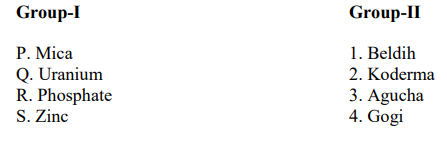
\includegraphics[width=0.7\textwidth]{figures/20.png}
\end{center}
\begin{enumerate}
    \item[(A)] P-2, Q-3, R-4, S-1
    \item[(B)] P-2, Q-4, R-1, S-3
    \item[(C)] P-4, Q-2, R-3, S-1
    \item[(D)] P-3, Q-1, R-4, S-2
\end{enumerate}
\vspace{0.5cm}

\questiona{Which one of the following corrections is always added during reduction of the observed gravity data?}{21}
\begin{enumerate}
    \item[(A)] Latitude
    \item[(B)] Free-air
    \item[(C)] Bouguer
    \item[(D)] Terrain
\end{enumerate}
\vspace{0.5cm}

\questiona{The magnitudes of the total geomagnetic field at the equator and pole are denoted by \(B_E\) and \(B_P\), respectively. Which one of the following is TRUE?}{22}
\begin{enumerate}
    \item[(A)] \(B_P \approx 4 B_E\)
    \item[(B)] \(B_P \approx 2 B_E\)
    \item[(C)] \(B_P \approx B_E\)
    \item[(D)] \(B_P \approx \frac{1}{2} B_E\)
\end{enumerate}
\vspace{0.5cm}

\questiona{Assume a flat earth with crustal thickness of 35 km and average crustal and upper mantle P-wave velocities of 6.4 km/s and 8.1 km/s, respectively. The minimum distance from the epicenter of a near surface earthquake at which Pn-waves are observed is \_\_\_\_\_ km.}{23}
\vspace{0.5cm}

\questiona{Given that the velocity of P-waves in a sandstone matrix is 5600 m/s and that in oil is 1200 m/s, the velocity of P-wave propagation in oil saturated sandstone with 30\% porosity is \_\_\_\_\_\_\_ m/s. (Use Wyllie time average equation.)}{24}
\vspace{0.5cm}

\questiona{If the total porosity of a soil is 20\%, its void ratio (\%) is \_\_\_\_\_\_\_\_\_.}{25}
\vspace{0.5cm}

\questionb{Which one of the following Himalayan lithounits predates India-Eurasia collision?}{26}
\begin{enumerate}
    \item[(A)] Kasauli sandstone
    \item[(B)] Rangit Pebble Slate
    \item[(C)] Annapurna granite
    \item[(D)] Lower Karewa sandstone
\end{enumerate}
\vspace{0.5cm}

\questionb{Which one of the following ore minerals shows internal reflection?}{27}
\begin{enumerate}
    \item[(A)] Orpiment
    \item[(B)] Magnetite
    \item[(C)] Pyrite
    \item[(D)] Molybdenite
\end{enumerate}
\vspace{0.5cm}

\questionb{Which one is CORRECT for the following equilibrium reaction between quartz and magnetite: \\[0.2cm]
\(\text{Si}^{16}\text{O}^{16} + \text{Fe}_3^{16}\text{O}_3^{18} \rightarrow \text{Si}^{16}\text{O}^{18} + \text{Fe}_3^{16}\text{O}_4\)?}{28}
\begin{enumerate}
    \item[(A)] \(1000 \ln \alpha = \Delta_{\text{qtz-mag}}\) where \(\alpha = K^{1/n}\) (K is the equilibrium constant at the specified temperature and n is a constant quantity)
    \item[(B)] \(1000 \ln \alpha = \Delta_{\text{qtz-mag}}\) where \(\alpha = K^n\) (K is the equilibrium constant at the specified temperature and n is the number of exchangeable atomic sites)
    \item[(C)] \(\frac{\ln \alpha}{1000} = \Delta_{\text{qtz-mag}}\) where \(\alpha = K^{1/n}\)
    \item[(D)] \(1000 \ln \alpha = \Delta_{\text{qtz-mag}}\) where \(\alpha = K^{1/n}\) and n is the number of exchangeable atomic sites
\end{enumerate}
\vspace{0.5cm}

\questionb{Match the modes of life (listed in Group I) with the corresponding bivalve genera (listed in Group II).}{29}
\begin{center}
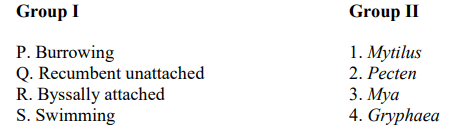
\includegraphics[width=0.7\textwidth]{figures/29.png}
\end{center}
\begin{enumerate}
    \item[(A)] P-4, Q-3, R-2, S-1
    \item[(B)] P-3, Q-4, R-1, S-2
    \item[(C)] P-2, Q-3, R-1, S-4
    \item[(D)] P-3, Q-1, R-4, S-2
\end{enumerate}
\vspace{0.5cm}

\questionb{Based on the hypothetical litholog given below that shows a continuous succession of sedimentary rocks, which one of the following statements is CORRECT?}{30}
\begin{center}
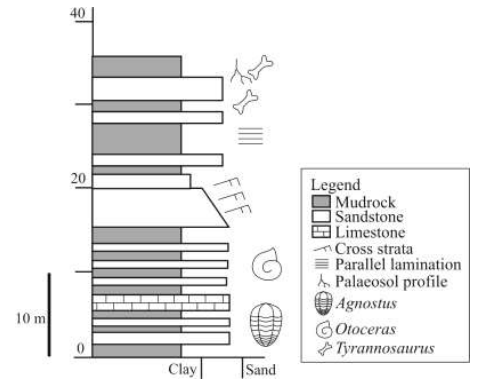
\includegraphics[width=0.5\textwidth]{figures/30}
\end{center}
\begin{enumerate}
    \item[(A)] The rocks range from Cambrian to Cretaceous and show change in depositional environment from marine to continental
    \item[(B)] The rocks range from Cambrian to Triassic and show change in depositional environment from marine to continental
    \item[(C)] The rocks range from Cambrian to Cretaceous and show change in depositional environment from continental to marine
    \item[(D)] The rocks are Palaeozoic in age and show change in depositional environment from marine to continental
\end{enumerate}
\vspace{0.5cm}

\questionb{Which one of the following cladograms shows the CORRECT interrelationships among the major groups of vertebrates?}{31}
\begin{center}
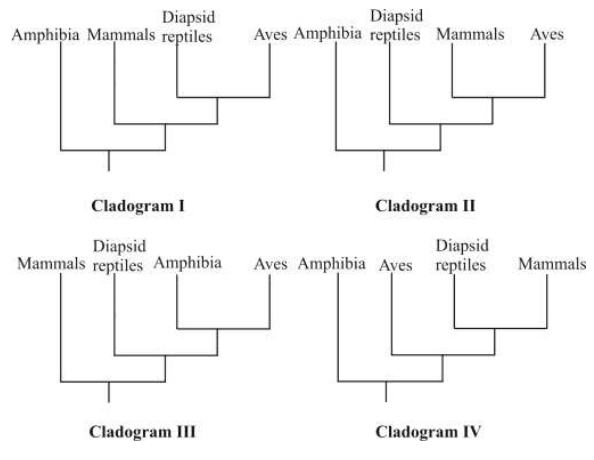
\includegraphics[width=0.5\textwidth]{figures/31}
\end{center}
\begin{enumerate}
    \item[(A)] Cladogram I
    \item[(B)] Cladogram II
    \item[(C)] Cladogram III
    \item[(D)] Cladogram IV
\end{enumerate}
\vspace{0.5cm}

\questionb{Which one of the following stratigraphic successions is in the CORRECT chronological order (from older to younger)?}{32}
\begin{enumerate}
    \item[(A)] Rajmahal, Dubrajpur, Barakar
    \item[(B)] Fenestella Shale, Muth Quartzite, Syringothyris Limestone
    \item[(C)] Bagh Bed, Lameta Formation, Deccan Traps
    \item[(D)] Singhbhum Granite, Kolhan Group, Older Metamorphic Gneiss
\end{enumerate}
\vspace{0.5cm}

\questionb{Match the items listed in Group I with their appropriate description listed in Group II.}{33}
\begin{center}
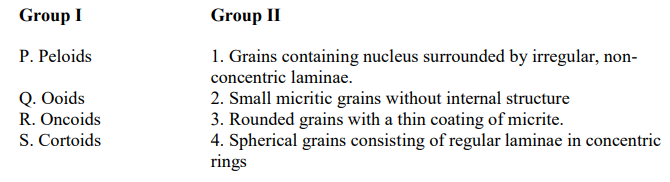
\includegraphics[width=0.8\textwidth]{figures/33.png}
\end{center}
\begin{enumerate}
    \item[(A)] P-3, Q-1, R-4, S-2
    \item[(B)] P-2, Q-4, R-1, S-3
    \item[(C)] P-3, Q-4, R-1, S-2
    \item[(D)] P-2, Q-3, R-4, S-1
\end{enumerate}
\vspace{0.5cm}

\questionb{Which one of the following is an image rectification technique?}{34}
\begin{enumerate}
    \item[(A)] Histogram equalization
    \item[(B)] Density slicing
    \item[(C)] Histogram normalization
    \item[(D)] Rubbersheeting
\end{enumerate}
\vspace{0.5cm}

\questionb{Match the items listed in Group I with those in Group II.}{35}
\begin{center}
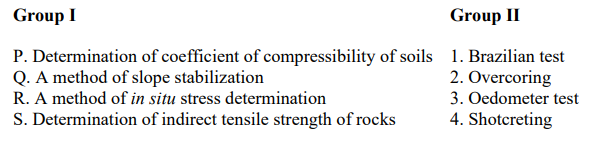
\includegraphics[width=0.7\textwidth]{figures/35.png}
\end{center}
\begin{enumerate}
    \item[(A)] P-4, Q-2, R-3, S-1
    \item[(B)] P-1, Q-4, R-2, S-3
    \item[(C)] P-3, Q-2, R-1, S-4
    \item[(D)] P-3, Q-4, R-2, S-1
\end{enumerate}
\vspace{0.5cm}

\questionb{Match the items listed in Group I with those listed in Group II.}{36}
\begin{center}
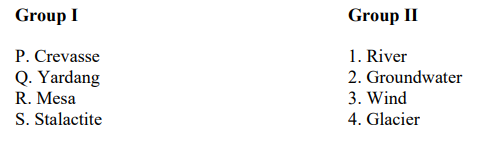
\includegraphics[width=0.7\textwidth]{figures/36.png}
\end{center}
\begin{enumerate}
    \item[(A)] P-4, Q-3, R-1, S-2
    \item[(B)] P-3, Q-1, R-4, S-2
    \item[(C)] P-4, Q-2, R-3, S-1
    \item[(D)] P-1, Q-2, R-3, S-4
\end{enumerate}
\vspace{0.5cm}

\questionb{In the hypothetical isobaric ternary liquidus projection diagram given below, solid phases A, B, C, D and E exist in equilibrium with liquid. The reaction taking place at the isobaric invariant point W is}{37}
\begin{center}
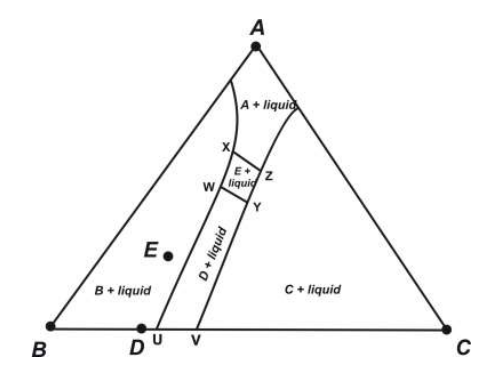
\includegraphics[width=0.5\textwidth]{figures/37}
\end{center}
\begin{enumerate}
    \item[(A)] Liquid (at W) = B + D + E
    \item[(B)] Liquid (at W) = A + B + D
    \item[(C)] Liquid (at W) + E = B + D
    \item[(D)] Liquid (at W) + B + D = E
\end{enumerate}
\vspace{0.5cm}

\questionb{Match the optical properties listed in Group I with the corresponding mineral in Group II.}{38}
\begin{center}
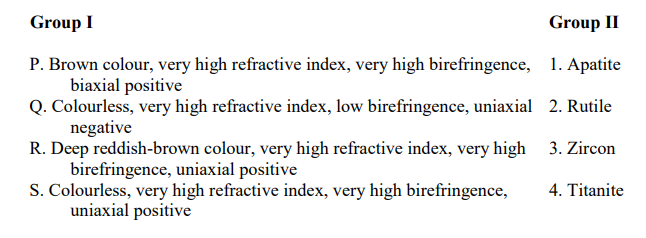
\includegraphics[width=0.7\textwidth]{figures/38.png}
\end{center}
\begin{enumerate}
    \item[(A)] P-4, Q-1, R-2, S-3
    \item[(B)] P-1, Q-2, R-4, S-3
    \item[(C)] P-3, Q-4, R-1, S-2
    \item[(D)] P-4, Q-1, R-3, S-2
\end{enumerate}
\vspace{0.5cm}

\questionb{The reaction \\[0.2cm]
muscovite + quartz = K-feldspar + sillimanite + water}{39}
\begin{enumerate}
    \item[(A)] takes place within the greenschist facies
    \item[(B)] takes place within the amphibolite facies
    \item[(C)] takes place within the eclogite facies
    \item[(D)] takes place within the granulite facies
\end{enumerate}
\vspace{0.5cm}

\questionb{Match the items listed in Group I with those in Group II.}{40}
\begin{center}
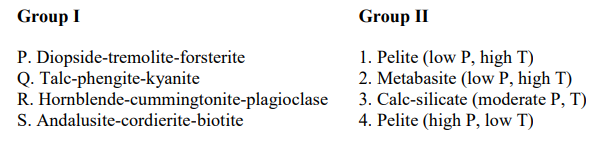
\includegraphics[width=0.7\textwidth]{figures/40.png}
\end{center}
\begin{enumerate}
    \item[(A)] P-3, Q-4, R-1, S-2
    \item[(B)] P-1, Q-2, R-4, S-3
    \item[(C)] P-3, Q-4, R-2, S-1
    \item[(D)] P-1, Q-2, R-3, S-4
\end{enumerate}
\vspace{0.5cm}

\questionb{The figure below is a schematic section showing the initial stages of development of a thrust fault (FF') having a typical ramp and flat geometry, with the thrust sheet being transported from east to west. With respect to the synform and antiform created in Stage 2, which one of the options below is CORRECT for the next increment of movement on the fault plane?}{41}
\begin{center}
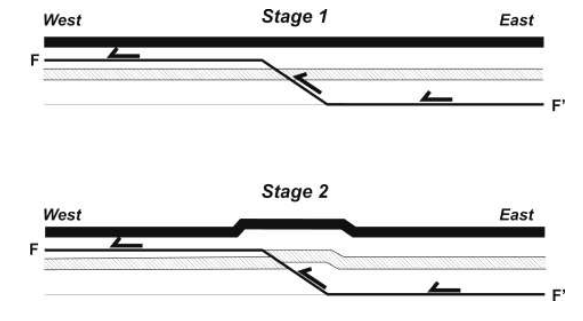
\includegraphics[width=0.7\textwidth]{figures/41}
\end{center}
\begin{enumerate}
    \item[(A)] The synform and the antiform will both move westward
    \item[(B)] The synform will remain in position, while the antiform will grow in amplitude
    \item[(C)] Both synform and antiform will grow in amplitude
    \item[(D)] The geometry will remain unchanged
\end{enumerate}
\vspace{0.5cm}

\questionb{Which one of the following is the CORRECT chronological sequence for Iron formations?}{42}
\begin{enumerate}
    \item[(A)] Algoma type > Superior type > Rapitan type > Minette type
    \item[(B)] Superior type > Algoma type > Rapitan type > Minette type
    \item[(C)] Rapitan type > Minette type > Algoma type > Superior type
    \item[(D)] Algoma type > Minette type > Superior type > Rapitan type
\end{enumerate}
\vspace{0.5cm}

\questionb{Assertion (a): High-temperature, low-pressure metamorphism occurs on the over-riding plate near convergent plate margins.\\
Reason (r): Partial melting in the mantle wedge generates magmas that rise to form the arc.}{43}
\begin{enumerate}
    \item[(A)] (a) is true but (r) is false
    \item[(B)] (a) is false but (r) is true
    \item[(C)] Both (a) and (r) are true and (r) is the correct reason for (a)
    \item[(D)] Both (a) and (r) are true and (r) is not the correct reason for (a)
\end{enumerate}
\vspace{0.5cm}

\questionb{Two coeval primary aqueous biphase fluid inclusions, X (liquid-rich) and Y (vapour-rich), occur in the same grain of the host mineral. Which one of the following situations most likely indicates boiling of the fluid?}{44}
\begin{enumerate}
    \item[(A)] X homogenizes to liquid and Y homogenizes to vapour at different temperatures
    \item[(B)] Both homogenize to liquid at the same temperature
    \item[(C)] Both homogenize to vapour at the same temperature
    \item[(D)] X homogenizes to liquid and Y homogenizes to vapour at the same temperature
\end{enumerate}
\vspace{0.5cm}

\questionb{During bench blasting in a quarry, 50 kg of an explosive with a yield of 5 MegaJoule/kg is required to break 100 m\(^3\) of marble. In this case, the energy expended in breaking a unit volume of marble in MegaNewton/m\(^2\) would be \_\_\_\_\_\_\_\_\_\_\_.}{45}
\vspace{0.5cm}

\questionb{The stretching lineation on the axial plane (S2) of a reclined fold on the S1 foliation makes an angle of \(30^\circ\) with the S1/S2 intersection lineation. The rake of the stretching lineation on the axial plane in degrees is \_\_\_\_\_\_\_.}{46}
\vspace{0.5cm}

\questionb{A basaltic magma has an initial nickel concentration of 300 ppm. Olivine crystallizes from this magma by equilibrium crystallization (Case I) or fractional crystallization (Case II). Then, the absolute value of the difference between the nickel concentrations of the liquids remaining after 25\% crystallization in these two cases is \_\_\_\_\_\_\_. (Use \( K_D^{\text{Ni, olivine/melt}} = 10 \))}{47}
\vspace{0.5cm}

\questionb{The difference in the number of faces in forms \{hkl\} and \{111\} in the holosymmetric class of the isometric system is \_\_\_\_\_\_\_.}{48}
\vspace{0.5cm}

\questionb{An inclined cylindrical confined aquifer has coefficient of permeability of 40 m/day. The horizontal distance between two vertical wells penetrating the aquifer is 800 m. The water surface elevations in the wells are 50 m and 45 m above a common horizontal datum. The absolute value of Darcy flux through the aquifer is \_\_\_\_\_\_\_ m/day.}{49}
\vspace{0.5cm}

\questionb{The mass and volume of a natural soil sample are 2.1 kg and \(1 \times 10^{-3}\) m\(^3\), respectively. When fully dried, the mass of the soil sample becomes 2 kg without any change in volume. Assuming the specific gravity of soil particles to be 2.5, and water density of 1000 kg/m\(^3\), the degree of saturation of the natural soil sample is \_\_\_\_\_\_\_\_\_\_ \%.}{50}
\vspace{0.5cm}

\questionb{For a granitic rock mass, joint set number (Jn) = 9, joint water reduction factor (Jw) = 1, joint alteration number (Ja) = 1, stress reduction factor (SRF) = 1, rock quality designation (RQD) = 84\%, and joint roughness number (Jr) = 3. The Q-value as per Barton’s Q-system of rock mass classification (year 1974) is \_\_\_\_\_\_\_.}{51}
\vspace{0.5cm}

\questionb{A sun synchronous satellite is at an altitude of 300 km and the spectrometer makes an angular coverage angle of \(12^\circ\). The Swath (GFOV) of the satellite is \_\_\_\_\_\_\_ km.}{52}
\vspace{0.5cm}

\questionb{The stability field boundary between two minerals A and B is linear with a positive slope in P-T space. The molar entropy of A and B are 85.5 and 92.5 J K\(^{-1}\), respectively, and their respective molar volumes are 35.5 and 38.2 cc. The slope of the phase boundary in P-T space is \_\_\_\_\_\_\_ bar K\(^{-1}\).}{53}
\vspace{0.5cm}

\questionb{Five moles of gas A (volume \(V_1\)) and three moles of gas B (volume \(V_2\)) were kept in separate containers. These two gases are completely transferred to a new container of volume V. Assuming isothermal condition, and that the work done is only mechanical, the entropy change of the system is \_\_\_\_\_\_\_ J K\(^{-1}\). (R = 8.3 J K\(^{-1}\) mol\(^{-1}\))}{54}
\vspace{0.5cm}

\questionb{The value of Eh corresponding to the upper limit of natural surface aqueous environment at pH of 8.0 is \_\_\_\_\_\_\_ V.}{55}
\vspace{0.5cm}




\vspace{5cm}
\begin{center}
\textbf{END OF THE QUESTION PAPER} \\
\rule{\textwidth}{0.5pt}
\end{center}

\end{document}
